\chapter{Caratterizzazione sperimentale di SiPM}\label{caratterizzazione_sipm}
\section{Analisi e funzionamento di un SiPM}
Il Silicon Photo Multiplier (SiPM) è un dispositivo elettronico che permette di rilevare radiazioni luminose con diversi livelli di intensità 
e di convertire questa grandezza fisica in corrente elettrica con la possibilità di rivelare singoli fotoni. Il SiPM è un dispositivo allo stato solido, basato cioè sull'uso di semiconduttori come materiali di costruzione 
(in questo caso il silicio), gode perciò di ottime proprietà quali una bassa tensione di alimentazione, insensibiltà ai campi magnetici, ottima 
robustezza meccanica e uniformità di risposta \cite{semiconductorcomponentsindustriesllc2011_2023_and9770}.
Come si può vedere dalla \autoref*{fig:sipm_adp_circuito}, il SiPM è composto da una matrice di fotodiodi, chiamati Single-Photon Avalanche Diode
(SPAD), che verranno analizzati a breve. I fotodiodi sono dispositivi a semiconduttore formati da una giunzione p-n (\autoref*{fig:adp}).
\begin{figure}[h!]
    \centering
    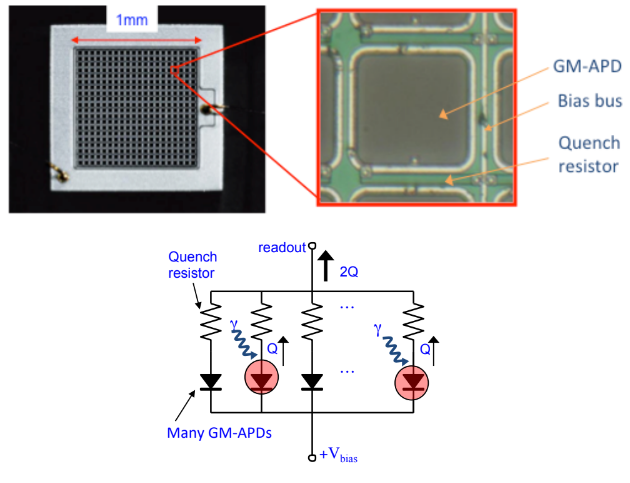
\includegraphics[width=.75\linewidth]{img/sipm_adp_circuito.png}
    \caption{Fotografia di un SiPM (sinistra) e di uno SPAD (destra) con il circuito equivalente (sotto) \cite{linssen_2023_eurizon}.}
    \label{fig:sipm_adp_circuito}
\end{figure}
\begin{figure}[h!]
    \centering
    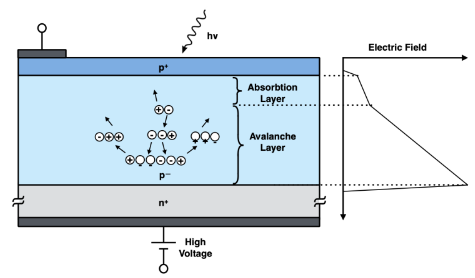
\includegraphics[width=.75\linewidth]{img/ADP.png}
    \caption{Schema strutturale di un SPAD, con a destra il grafico che descrive l'andamento dell campo elettrico avvicinandosi al catodo \cite{linssen_2023_eurizon}.}
    \label{fig:adp}
\end{figure}

La giunzione p-n che realizza il fotodiodo è responsabile della generazione della corrente elettrica. Quando un 
fotone colpisce il silicio drogato presente nel fotodiodo, trasferisce la sua energia agli elettroni che passano dalla banda di valenza 
a quella di conduzione creando una lacuna positiva. Applicando al dispositivo una tensione di polarizzazione inversa, con tensione
al catodo maggiore di quella all'anodo, gli elettroni sono attratti verso il catodo e le lacune verso l'anodo creando così una corrente
all'interno del fotodiodo. Il valore della corrente è proporzionale all'energia trasportata dal fotone, a sua volta inversamente 
proporzionale alla lunghezza d'onda secondo l'equazione
\begin{equation}
    E = \frac{h}{\lambda}
    \label{eq:energia_onde}
\end{equation}
dove $h$ è la costante di Planck e $\lambda$ la lunghezza d'onda. Quando si ha una tensione tra anodo e catodo sufficientemente grande
avviene un fenomeno chiamato ionizzazione a impatto, in cui una carica elettrica acquista sufficiente energia cinetica da creare coppie
di cariche secondarie, che a cascata innescano altre ionizazzioni a impatto, amplificando così la corrente generata da
un singolo fotone. In questa condizione il fotodiodo si trova in regione di break down ed è estremamente conduttivo. Questo processo è 
chiamato scarica Geiger e un fotodiodo che opera in questa modalità è detto SPAD. Una volta che la corrente 
scorre in questi dispositivi può essere necessario fermarla, per farlo si collega una resistenza, chiamata resistenza di quenching 
($R_Q$) in serie al fotodiodo, che limita la corrente assorbita dal diodo nella regione di break down, abbassando così la tensione applicata
ai capi del fotodiodo ad un valore inferiore a quello che permette il processo di polarizzazione a cascata, riportando il diodo nella
condizione di rilevare altri fotoni. È importante notare che, nel SiPM, ogni sottocircuito SPAD-$R_Q$, chiamato microcella, è indipendente, 
quindi ogni volta che avviene la ionizzazione a cascata, questa è isolata al solo fotodiodo innsecato \cite{semiconductorcomponentsindustriesllc2011_2023_and9770}. Le altre microcelle, nel caso di 
arrivo di un singolo fotone, restano disponibili per l'attivazione. Questa configurazione consente di distinguere radiazioni luminose di intensità 
diverse. Infatti un'intensità maggiore comporta un numero di fotoni maggiore e quindi l'attivazione contemporanea di più microcelle, le cui correnti 
in uscita si sommano a formare una corrente d'uscita dal SiPM maggiore.
Nella \autoref*{fig:sipm_schematico_corrente} è possibile osservare l'andamento della corrente che scorre nel fotodiodo in funzione del tempo 
insieme alla caratteristica I-V in cui sono descritte le regioni di funzionamento. La corrente che scorre nel fotodiodo, quando questo viene
attraversato dal fotone,raggiunge il suo valore massimo in un tempo inferiore a \SI{1}{\nano\second} per poi diminuire con una costante di tempo
pari a $\tau_f=R_QC_D$, dove $C_D$ è la capacità del volume di valanga, propria di ogni SPAD. Il processo appena descritto avviene solo se viene
applicata una tensione di polarizzazione inversa ai capi del fotodiodo $V_\text{bias}>V_B$ dove $V_B$ è la tensione di soglia propria del fotodiodo, 
come viene mostrato nella figura a destra: a partire dal valore di $V_\text{bias}>V_B$ viene innsecato il ciclo di funzionamento a cascata della microcella \cite{linssen_2023_eurizon}.  
\begin{figure}[h!]
    \centering
    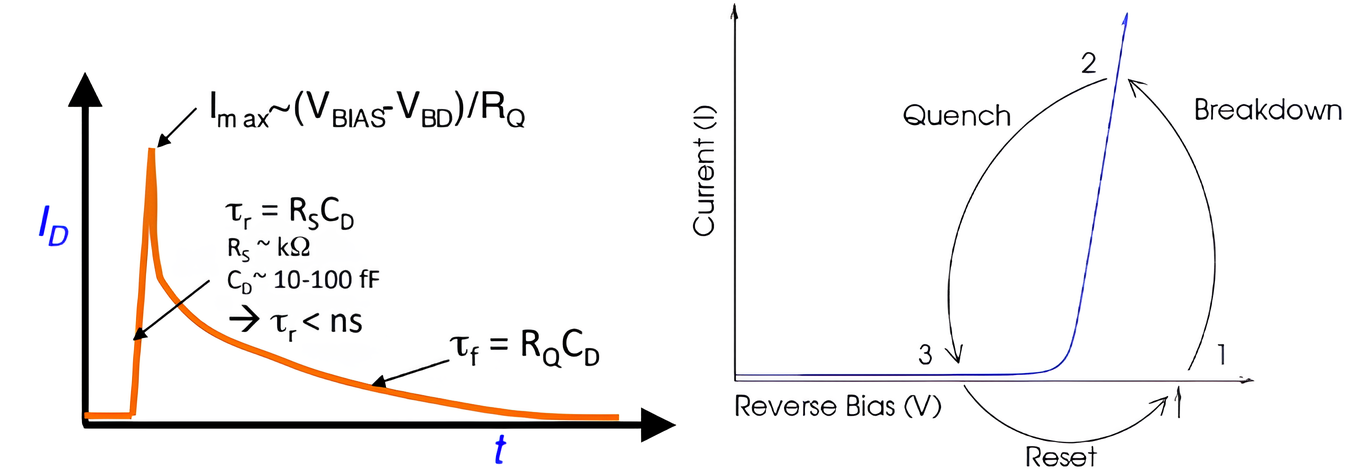
\includegraphics[width=1\linewidth]{img/ciclo_fotodiodo_corrente.png}
    \caption{Andamento nel dominio del tempo del ciclo breakdown-quench-reset (sinistra) e regioni di funzionamento nella
    caratteristica I-V (destra). In quest'ultima immagine il valore $V_B$ è indicato dalla freccia tra Reset e Breakdown.}
    \label{fig:sipm_schematico_corrente}
\end{figure}

Il SiPM viene utilizzato in molte applicazioni, come nel caso preso in esame in questo lavoro, in combinazione con un altro dispositivo 
chiamato scintillatore. Uno scintillatore è costituito da un materiale che emette impulsi di radiazione luminosa quando viene attraversato da 
particelle ad alta energia.
Questa configurazione permette di avere, al passaggio di un muone attraverso lo scintillatore, una radiazione luminosa in uscita da quest'ultimo 
che viene poi rilevata dal SiPM e convertita in una grandezza elettrica. Il tipo di SiPM utilizzato e il suo schema circuitale sono mostrati nella \autoref*{fig:sipm_schema_board}
\begin{figure}[h!]
    \centering
    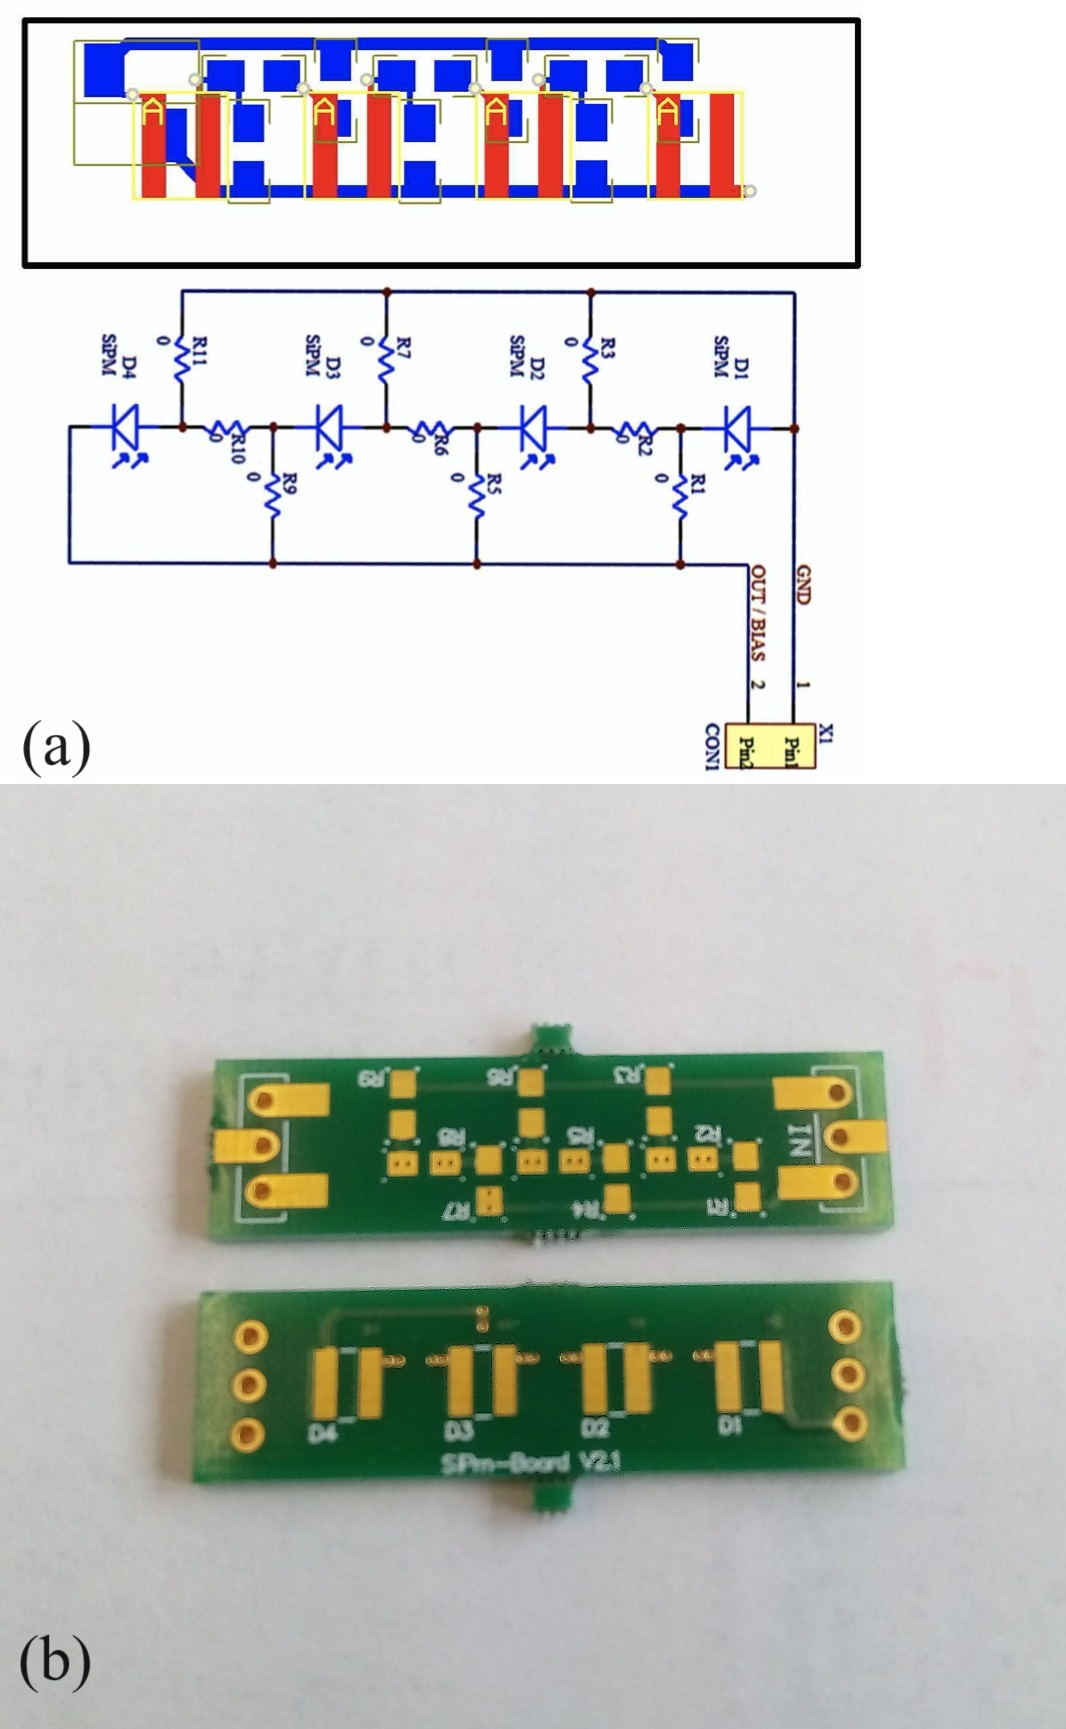
\includegraphics[width=.75\linewidth]{img/sipm_schema+board.jpg}
    \caption{a) Schematico della SiPM board usata nel progetto MuonPi. b) Fotografia di un SiPM \cite{muonpiwikicontributors_2017_sipm}.}
    \label{fig:sipm_schema_board}
\end{figure}

Il SiPM è un dispositivo che ha bisogno di alimentazione per poter funzionare, perciò il primo passo da seguire per allestire 
il circuito funzionante è caratterizzare il SiPM, stabilire cioè quale deve essere il valore di tensione da fornire affinché la giunzione p-n dei
fotodiodi operi nella regione di funzionamento corretta. Il valore della tensione di alimentazione deve essere quindi maggiore del valore di soglia 
del fotodiodo.
\section{Descrizione del setup di misura}\label{descrizione_setup}
Per determinare la tensione di alimentazione e la polarità del dispositivo, si utilizza un dispositivo che possa fornire una tensione 
controllabile, in questo caso è stato utilizzato un dispositivo chiamato DC Power Analyzer (Keysight N6705C DC Power Analyzer) che è in grado di 
fornire e misurare una tensione in corrente continua stabile ad un circuito cui è collegato. L'utilizzo di questo dispositivo permette anche il 
controllo da remoto con un calcolatore attraverso la comunicazione USB.
 Il power supply utilizzato è dotato di quattro canali utilizzabili sia in input che in output. In questo caso è 
stato utilizzato solo uno dei quattro canali in configurazione output. In questo modo è possibile impostare con precisione il valore di tensione e 
la corrente massima erogabile dal power supply. La configurazione completa è quella mostrata nella \autoref*{fig:setup_sipm}.
\begin{figure}[h!]
    \centering
    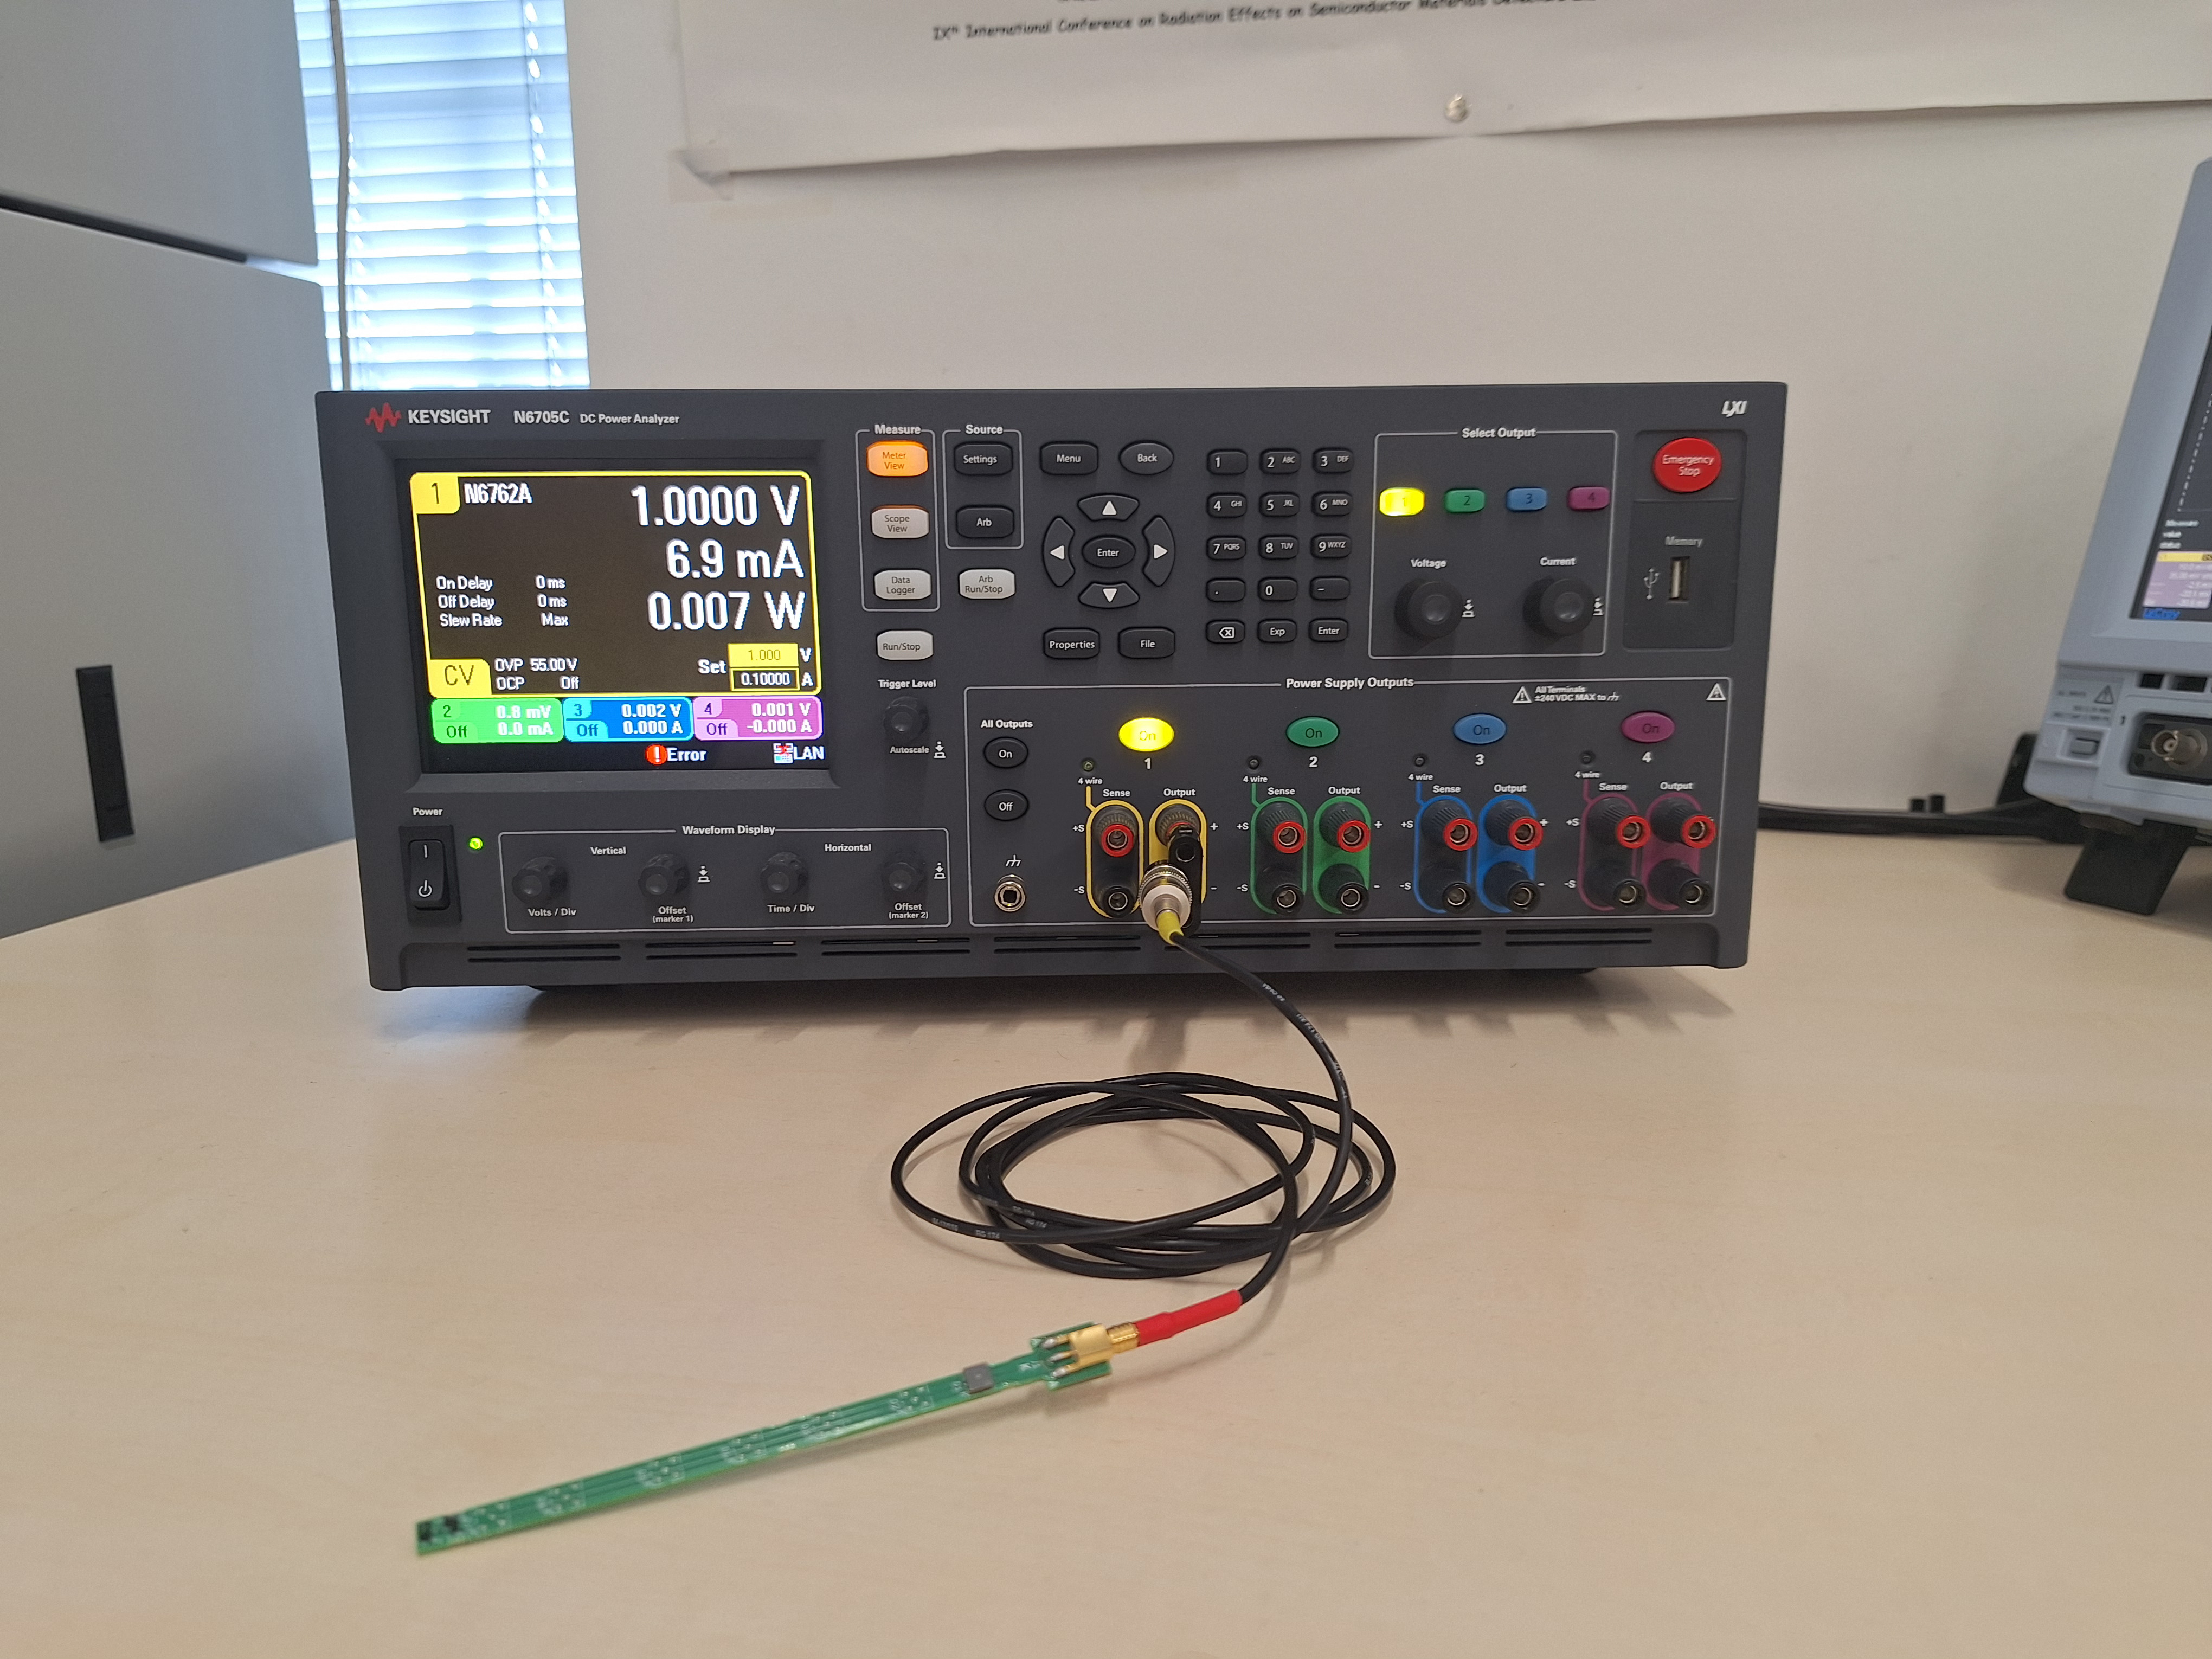
\includegraphics[width=.75\linewidth]{img/setup_sipm.jpg}
    \caption{Setup utilizzato per determinare la caratteristica tensione corrente del SiPM. In primo piano il SiPM collegato attraverso un cavo di 
    tipo BNC con connettore Lemo al DC Power Analyzer che si vede in secondo piano. Sul display di quest'ultimo si notano i valori di tensione e 
    corrente erogati.}
    \label{fig:setup_sipm}
\end{figure}
 Per facilitare la comunicazione, si è deciso di realizzare un testbench software in linguaggio Python data la vasta 
disponibilità di librerie e codici. Usando il modulo \texttt{pyvisa}, è possibile conoscere e controllare tutti i dispositivi di misura
connessi al calcolatore che esegue il codice indipendentemente dalla loro interfaccia di comunicazione. Utilizzando questo modulo è quindi possibile 
controllare il DC Power Analyzer accendendo o spegnendo un canale e leggendo o scrivendo il livello di tensione e di corrente in uscita dal canale. 
Sono state create quindi delle funzioni per facilitare questo processo.
 Con questi strumenti è possibile, sempre utilizzando un codice Python, procedere con la caratterizzazione del SiPM.
La caratterizzazione è un processo il cui obiettivo è stabilire le caratteristiche che descrivono il comportamento di un dospositivo elettronico.
Nel caso del SiPM, si vuole stabilire l'andamento della caratteristica tensione-corrente (comunemente indicata come caratteristica I-V) da cui è 
possibile dedurre la soglia minima di funzionamento, la funzione di trasferimento, cioè la legge, che lega la tensione di alimentazione con la 
massima corrente erogata e la resistenza di quenching. Per ottenere questi dati, si varia la tensione erogata dal DC Voltage Analyzer partendo da 
\SI{0}{\milli\volt} e con uno step di \SI{10}{\milli\volt} ogni \SI{2}{\second} fino al valore di \SI{1}{\volt}, oltre il quale il SiPM 
potrebbe non funzionare più correttamente. A questo punto, si misurano la corrente erogata dal SiPM e la tensione applicata dal power supply usando 
il modulo \texttt{pyvisa}. I dati ottentuti vengono salvati su un file \texttt{csv} grazie all'omonimo modulo di Python. Le misure vengono poi
utilizzate per la costruzione del grafico I-V disegnato dall'interfaccia \texttt{Pyplot} presente nella liberia \texttt{Matplotlib}.
\section{Risultati delle misure effettuate}
Usando il setup descritto nella \autoref*{descrizione_setup}si ottiene l'andamento indicato nella \autoref*{fig:char_iv}.
\begin{figure}[h!]
    \centering
    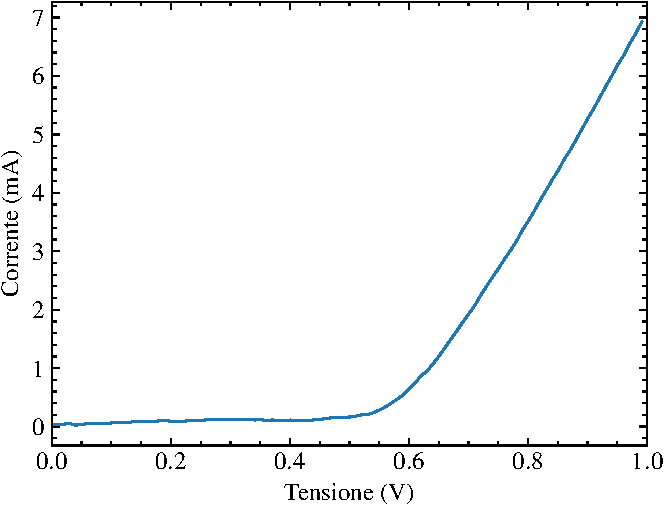
\includegraphics[width=.75\linewidth]{img/char_IV.pdf}
    \caption{Caratteristica tensione-corrente del SiPM misurata tra \SI{0}{\volt} e \SI{1}{\volt} con il solo SiPM collegato al DC Power Analyzer}
    \label{fig:char_iv}
\end{figure}

Osservando il grafico si nota un andamento lineare a partire da circa \SI{0,7}{\volt}, mentre per valori più bassi si ha
una corrente pari a circa \SI{0}{\ampere}, condizione che si verifica quando il SiPM è spento. Il valore \SI{0,7}{\volt} è quindi la 
soglia della funzione di trasferimento, cioè il minimo valore di tensione che si può fornire al SiPM per far sì che questo funzioni. 
Per ottenere la funzione di trasferimento nella regione in cui si ha andamento lineare, cioè la regione in cui il SiPM è attivo, da cui poi 
è possibile ricavare il valore della resistenza di quenching, si filtra il dataset includendo solo le misure a tensione maggiore di \SI{0,7}{\volt}. 
È utile in questi casi snellire il dataset eliminando una misura su due per ottenere risultati più simili alla realtà.
Il modulo di Python \texttt{scipy} permette di effetuare entrambe queste operazioni. A questo punto si effettua un'interpolazione lineare 
usando la funzione fornita sempre dal modulo \texttt{scipy} per ottenere il coefficente angolare e la quota del modello lineare che descrive la 
caratteristica I-V. I valori sono indicati nella \autoref*{fig:char_iv_filtered} che mostra graficamente la parte lineare della
caratteristica I-V.
\begin{figure}[h!]
    \centering
    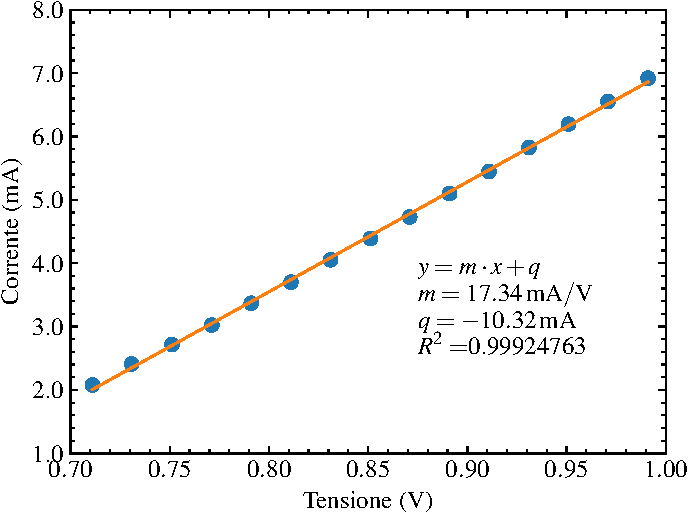
\includegraphics[width=.75\linewidth]{img/char_IV_filtered.pdf}
    \caption{Caratteristica tensione-corrente del SiPM misurata tra \SI{0,7}{\volt} e \SI{1}{\volt} con il solo SiPM collegato al DC Power Analyzer, si apprezza l'andamento lineare e la corrispondenza tra modello lineare e risultati empirici oltre ai valori di coefficente angolare e quota del modello.}
    \label{fig:char_iv_filtered}
\end{figure}
Uno strumento utile per stabilire la bontà del modello statistico utilizzato è il coefficente di determinazione $R^2$, che si ottiene direttamente
usando la funzione fornita dal modulo \texttt{scipy}. In questo caso, il valore di $R^2=0.999$ ci permette di affermare che il modello
lineare utilizzato rappresenta in modo ottimo il reale andamento dei dati.
Per ricavare la resistenza di quenching ($R_Q$), è sufficiente osservare che il grafico nella \autoref*{fig:char_iv_filtered} si riferisce ad una regione
in cui si ha una proporzionalità diretta tra tensione è corrente. Dalla \autoref*{fig:sipm_schematico_corrente} si vede che la regione in cui ciò
avviene è la regione di quench. Essendo tensione e corrente proporzionali, seguono quindi la prima legge di Ohm:
\begin{equation}
    V = R \cdot I
    \label{eq:legge_ohm}
\end{equation}
L'equazione ottenuta attraverso l'interpolazione lineare ci permette di esprimere la corrente in funzione della tensione, è cioè l'inverso
della legge di Ohm. Ne deriva che
\begin{equation}
    m = \frac{dI}{dV}
    \label{eq:slope}
\end{equation}
mentre la resistenza di quenching si può calcolare come
\begin{equation}
    R_Q= \frac{dV}{dI}=\frac{1}{m}=\frac{1}{\SI{17,34}{\milli\ampere/\volt}}=\SI{57,67}{\ohm}
    \label{eq:resistenza_quenching}
\end{equation}
L'equazione \autoref*{eq:resistenza_quenching} per calcolare la $R_Q$ poteva essere dedotta anche analizzando il circuito mostrato in 
\autoref*{fig:circuito_microcella}. Effettuando un bilanciamento di correnti al nodo $OUT$ si ottiene l'\autoref*{eq:risoluzione_circuito1}, 
da cui si ricava la \autoref*{eq:risoluzione_circuito2}, che è equivalente a quanto ottenuto nell'\autoref*{eq:resistenza_quenching}
\begin{equation}
    I_D=\frac{V_\text{bias}}{R_Q}
    \label{eq:risoluzione_circuito1}
\end{equation}
\begin{equation}
    R_Q=\frac{V_\text{bias}}{I_D}
    \label{eq:risoluzione_circuito2}
\end{equation}
\begin{figure}[h!]
    \centering
    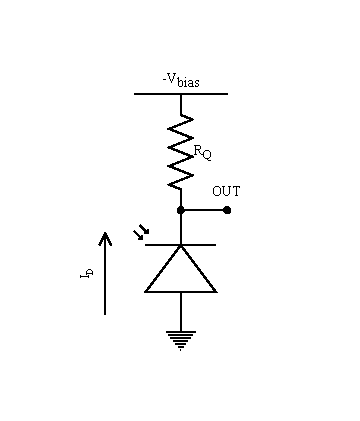
\includegraphics[width=0.65\linewidth]{img/circuito_microcella.pdf}
    \caption{Schematico di una microcella}
    \label{fig:circuito_microcella}
\end{figure}
